%________________________________________________________________________________________________
\documentclass{beamer}
%________________________________________________________________________________________________
\usepackage[french]{babel} 
\usepackage[utf8]{inputenc} 
\usepackage[T1]{fontenc} 
\usepackage{graphicx}
\usepackage[utf8]{inputenc}
\usepackage{fancyhdr}
\usepackage{geometry}
\usepackage{tabularx,tabulary}
\usepackage{movie15}
%________________________________________________________________________________________________
\title{3I013 Réunion du 29 Mars 2019}
\author{Nicolas CASTANET\\Maël FRANCESCHETTI\\Daoud KADOCH\\Fabien MANSON\\}
%________________________________________________________________________________________________
%ce theme est le plus clean de Beamer le truc a ne pas utiliser c'est 'Warsaw'
\usetheme{default}
%suppression de la barre de navigation inutile
\setbeamertemplate{navigation symbols}{}
\setbeamertemplate{frametitle}[default][center]

%\logo{
\includegraphics[height=0.5cm]{logo_sorbonne.png}}

%________________________________________________________________________________________________
\addtobeamertemplate{footline}{
	\begin{flushright}
	\vbox{\insertframenumber/\inserttotalframenumber}
	\end{flushright}}

%________________________________________________________________________________________________
\begin{document}


	\begin{frame}
		\begin{center}
		\date{}
		\maketitle
		\end{center}
	\end{frame}
	
	
	
	\begin{frame}
		\section{}
		\begin{center}
		\frametitle{Sommaire}
		\tableofcontents{}
		\end{center}
	\end{frame}
	
	
	
	\begin{frame}
		\section{Problème}
		\begin{center}
		\frametitle{Objectifs}
		\begin{itemize}
		    \item Le client souhaite effectuer des rondes avec un drone Bebop 2\\
		    \item Le drone doit voler de manière autonome en suivant un plan de vol prédéfini \\
		    \item Le retour vidéo du drone doit être redirigé à un iPod touch qui sera placé dans un masque FPV pour permettre à l'utilisateur de voir comme s'il était à la place du drone\\
		\end{itemize}
		   
		\end{center}
	\end{frame}
	
	\begin{frame}
		\section{Problème}
		\begin{center}
		\frametitle{Cas d'utilisation}
		\begin{enumerate}
		    \item Démarrage du drone\\
		    \item Lancement de l'application PC\\
		    \item Saisie du plan de vol à l'aide du composant dédié (carte intéractive)\\
		    \item Connexion du PC au wifi du drone
		    \item Connexion de l'iPod au réseau local et démarrage de l'application sur l'iPod
		    \item Mise en place de l'iPod dans le masque FPV
		    \item Demarrage de la ronde depuis l'iPod ou le PC
		    \item Arrêt d'urgence si besoin
		\end{enumerate}
		   
		\end{center}
	\end{frame}
	
	\begin{frame}
		\section{Solution}
		\begin{center}
		\frametitle{Architecture Matérielle}
		%\subsection{Contraintes}
        %\framesubtitle{Les solutions}
       
        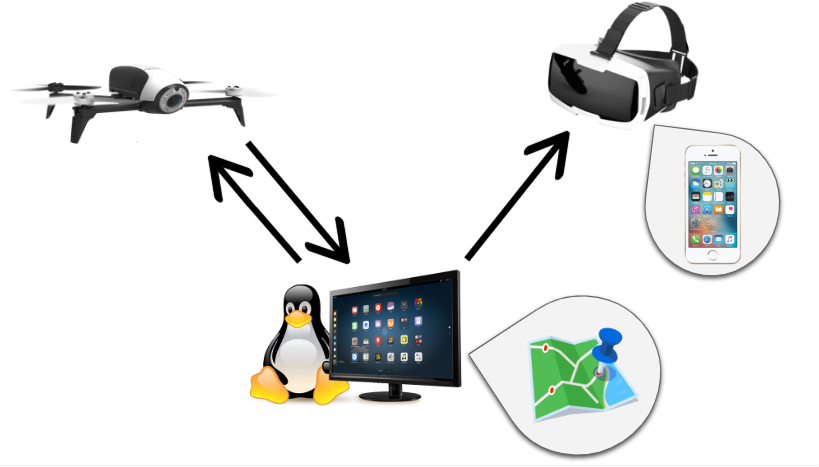
\includegraphics[scale=0.6]{shcema_archi.png}
		\end{center}
	\end{frame}
	
	\begin{frame}
		\section{Solution}
		\begin{center}
		\frametitle{Architecture Logicielle}
		%\subsection{Contraintes}
        %\framesubtitle{Les solutions}
       
        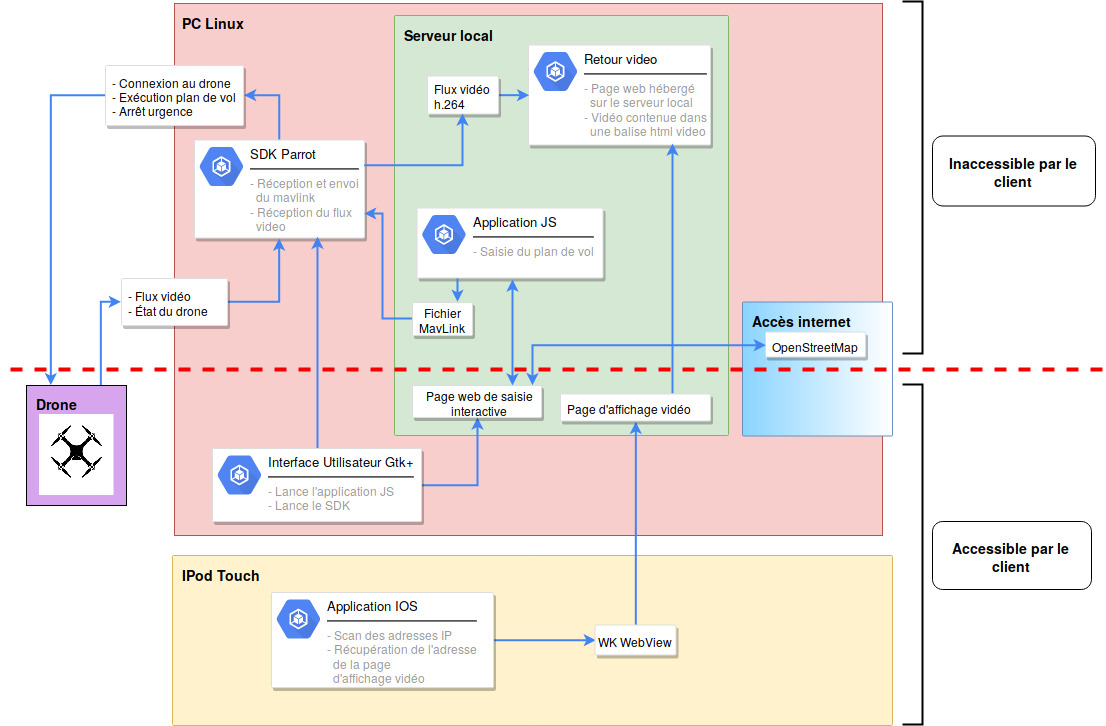
\includegraphics[scale=0.3]{Architecture_logicielle_v2.jpg}
		\end{center}
	\end{frame}
	

	
	
	\begin{frame}
		\section{Avancement}
		\begin{center}
		\frametitle{Tests effectués}
           	\begin{itemize}
           	    \item Saisie d'un plan de vol enregistré au format Mavlink
                \item Connexion au drone
                \item Envoi d'un fichier Mavlink avec le SDK
                \item Initialisation des paramètres pour le vol autonome
                \item Exécution du plan de vol enregistré sur le drone en totalité.
                 \item Arrêt d'urgence
                \item Essais d'émission d'un flux vidéo depuis un serveur vers un iPod
            \end{itemize}
		\end{center}
	\end{frame}
	
	\begin{frame}
		\section{Avancement}
		\begin{center}
		\frametitle{Etat d'avancement}
         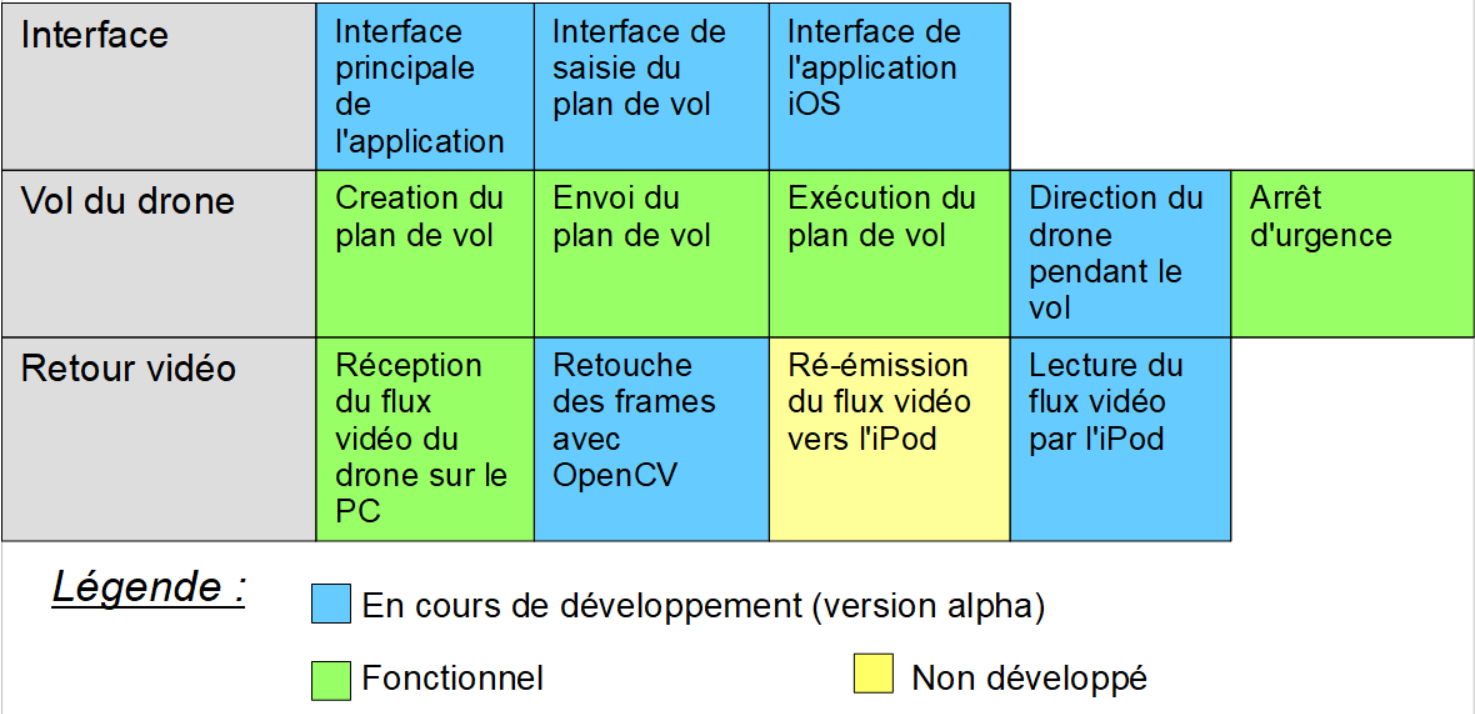
\includegraphics[scale=0.35]{Avancement_projet.PNG}
        \end{center}
	\end{frame}
	
	
	
	\begin{frame}
		\section{Avancement}
		\begin{center}
		\frametitle{Problèmes rencontrés}
	    	Résolus :
             \begin{itemize}
                \item Calibration du drone après chaque arrêt d'urgence (choc ou inclinaison trop forte du drone).
                \item Direction du drone durant le trajet.
            \end{itemize}
            En cours :
            \begin{itemize}
                \item Perte du signal GPS
                \item Retouche des frames du flux vidéo pour le split screen
                \item Ré-émission du flux vidéo par le serveur
            \end{itemize}
		\end{center}
	\end{frame}
	
	
\end{document}
